
\chapter{Bluetooth Module Design}
% \stepcounter{chapter}\addcontentsline{toc}{chapter}{Incremental Sigma-Delta Modulator}

\section{Introduction}


An Antenna design and analysis are crucial in a wireless network that transmits and receives information through electromagnetic wave radiation in open space.
Modern Antenna and RF design techniques more often testified against size, power, flexibility, radiation patterns, efficiency, etc...
It is very unusual to use a wide variety of RF fundamental design techniques even though the usage of silicon and power is different because the fundamentals of RF design are most rigorous and robust from decades, hence RF fundamentals and design techniques remain intact. Nevertheless, modern RF applications demand to emphasize efficiency and power requirements, so this requirement needs some special RF Design treatments.
Chapter .3 gives the extravagance of PCB antenna design practices, general guidelines for grounding, PCB stacking, spacings and via holes, etc. Matching networks in RF design are extremely important to increase the efficiency of the Antenna and RF line, so it is also explored in the same chapter how to pick the passive components for RF Antenna matching such as capacitors and inductors.

%%%%%%*********************************************************%%%%%%%
%%%%%%*************************New Section*********************%%%%%%%
%%%%%%*********************************************************%%%%%%%
\section{Antenna Basics :}

An Antenna is a piece of metal exposed to free space. A piece of conductor behaves like an antenna when its length is a certain ratio or multiple of the wavelength of the signal. This scenario is expressed as "resonance", where the antenna radiates the electrical energy to the open space.




\begin{figure}[h]
	\centering
	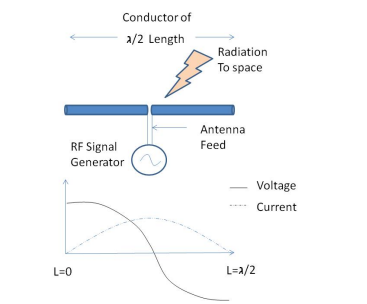
\includegraphics[width=0.7\textwidth]{Chap03/Figures/Basic_Antenna.PNG}
	\caption{Basic Diploe Antenna}
	\label{BASIC_ANTENNA}
\end{figure}

Fig.1  shows the diploe antenna whose length is  $\lambda/2$ and the fed has an input impedance of $50\omega$.
Dipole antennas are the most basic antennas that have been used for broadcasting.
In the Millennial age of technology, dipole antennas have been bulky and heavy, thanks to the PCB technology, which made diploe antennas extremely simple in construction and this became the center of attraction for the Bluetooth application in the modern era.
Although diploe antennas are extremely comfortable for PCB we still face hurdles to manage proper grounding for the antenna..which can be addressed through quarter-wave antennas.
The quarter-wave antennas have half of the length of the dipole antennas  $\lambda/4$ their popularity became exponential because of the fed which can be single-ended.
A single-ended feed to the antenna made life much easier to make a wide range of ground planes and better matching.

%%%%%%%%%%%%%%%%%%%%%%%%%%%%%%%%%%%%%%%%%%%%%%%%%%%%%%%%%%%%%%%%%%%%%%%%%%%%%%%%%%%%%
\subsection{Antenna Types:}

As discussed in the previous section quarter wavelength antennas can be more effective on the PCB because of their fed and ground plane management on PCB.
Depending on the antenna dimensions and the shape antennas fall into different technologies namely FM, AM, Bluetooth, and wifi son on.
Since the eccentric part of this chapter discusses the Bluetooth antenna design and guidelines, we can broadly classify three types of antennas. as Follows :

\subsubsection{Wire Antenna :}
These types of antennas are just a piece of wire extended over the PCB in open space, whose length is matched to $\dfrac{\lambda}{4}$ on the ground plane.
In general, these antennas are fed by a $50\omega$ matching transmission line, a Wire antenna gives a top-notch performance and supports a wide range of frequencies because of its three-dimensional exposure in open space.
The shape of the wire antennas can be loop, wire, or helix.. depending on the application the shape is changed.

\begin{figure}[h]
	\centering
	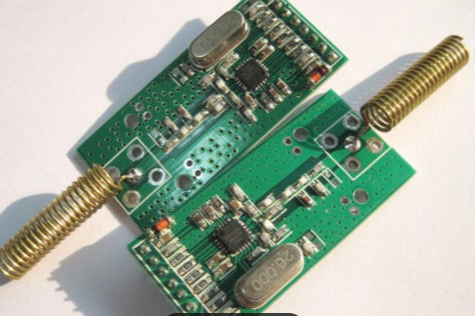
\includegraphics[width=0.4\textwidth]{Chap03/Figures/Wire_antenna.PNG}
	\caption{Wire Antenna}
	\label{WIRE_ANTENNA}
\end{figure}


\subsubsection{ PCB Antenna :}Constructively this type of antenna is copper traces
that are etched on the PCB. The Traces can be Zig-Zag, straight, MIFA, Meandered type, F-type, or Zip track so on.,
the shape of the antenna is chosen based on the antenna type and the space constraints on the PCB. PCB Antennas have only two-dimensional freedom, therefore certain guidelines are needed for the PCB antenna design due to the space constraints and poor quality of PCB stack-up.
The space constraints of the PCB antennas lead to less efficiency compared with wire antennas nonetheless PCB antennas are cost-effective.
In short manufacturing comfortability and its wireless range is ravishing for Bluetooth applications.

\begin{figure}[h]
	\centering
	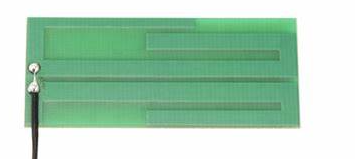
\includegraphics[width=0.4\textwidth]{Chap03/Figures/PCB_Antenna.PNG}
	\caption{PCB Antenna}
	\label{PCB_ANTENNA}
\end{figure}


\subsubsection{ Chip Antenna :} This is a Small form factor IC that is in-house with a ceramic package or some metal case.
These antennas are handier in terms of space management on the board and internally their impendence is very well managed.
A chip antenna can also take an advantage of three-dimensional freedom for radiation similar to wire antennas.
Refer to figure 10 for the Nordic Bluetooth module having a chip antenna.
It's true that chip antennas can gain upper hand in size and radion pattern on the contrary power handling capacity of the chip antenna is very minimal.
\begin{figure}[h]
	\centering
	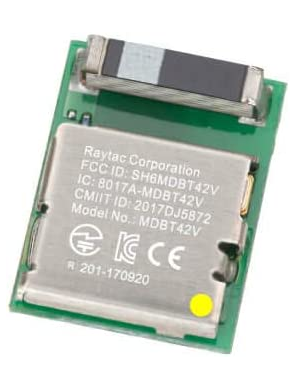
\includegraphics[width=0.4\textwidth]{Chap03/Figures/Chip_Antenna.PNG}
	\caption{Chip Antenna}
	\label{CHIP_ANTENNA}
\end{figure}



\subsection{Antenna Parameters}

The following section gives some key antenna performance parameters.

\subsubsection{Return loss :}

The return loss of an antenna signifies how well the antenna is matched to the 50-Ω transmission line (TL), shown as a signal feed in Figure \ref{fig:ANTENNA_RETUNRNLOSS}. The TL characteristic impedance is typically 50 Ω, although it could be a different value. The industry standard for commercial antennas and testing equipment is 50-Ω impedance, so it is most convenient to use this value \cite{AN91445}. \\
	
\indent  Return loss indicates how much of the incident power is reflected by the antenna due to mismatch (Equation \ref{eq:Antenna_Returnloss}).
An ideal antenna when perfectly matched will radiate the entire energy without any reflection. If the return loss is infinite, the antenna is said to be perfectly matched to the TL, as shown in Figure \ref{fig:ANTENNA_RETUNRNLOSS}. S11 is the negative return loss expressed in decibels. In most cases, a return loss ≥ 10 dB (equivalently, S11 ≤ –10 dB) is considered sufficient. Table \ref{tb:ANTENNA_RETURNlOSS_TABLE} relates the return loss (dB) to the power reflected from the antenna (percent). 
A return loss of 10 dB signifies that $90\%$ of the incident power goes into the antenna for radiation \cite{AN91445}.

\begin{equation}\label{eq:Antenna_Returnloss}
    \begin{split}
        Returnloss(db) = 10 \times \log( \frac{Pincident}{Preflected})
    \end{split}
\end{equation}

\begin{figure}[h]
	\centering
	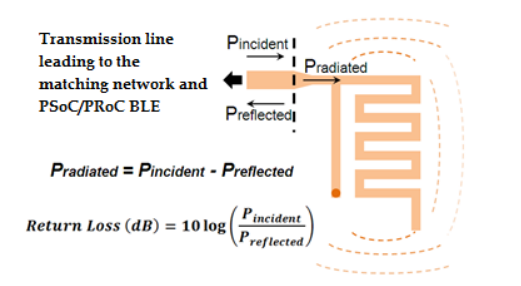
\includegraphics[width=0.65\textwidth]{Chap03/Figures/Antenna_ReturnLoss.PNG}
	\caption{Antenna Return loss}
	\label{fig:ANTENNA_RETUNRNLOSS}
\end{figure}

\begin{table}[h]
	\label{tb:ANTENNA_RETURNlOSS_TABLE}
	\begin{tabular}{|c|c|c|c| }
		\hline 
		S11 (dB) & Return Loss (dB) & Preflected/Pincident $(\%)$ & Pradiated/Pincident (\%) \\ 
		\hline
		–20 &20 &1 &99\\
		\hline
		–3 &3 &50 &50\\
		\hline
		–10 &10 &10& 90\\
		\hline
		–1 &1 &79 &21\\
		\hline
	\end{tabular}
	\caption{Return Loss and Power reflected from antenna}
\end{table}



\subsubsection{Bandwidth :}

Bandwidth indicates the frequency response of an antenna. It signifies how well the antenna is matched to the 50-Ω transmission line over the entire band of interest, that is, between 2.40 GHz and 2.48 GHz for BLE applications \cite{AN91445}.\\

	\begin{figure}[h]
		\centering
		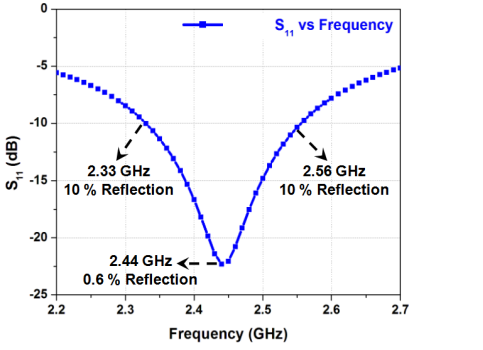
\includegraphics[width=0.65\textwidth]{Chap03/Figures/Antenna_Bandwidth.PNG}
		\caption{Antenna Bandwidth}
		\label{fig:ANTENNA_BANDWIDTH}
	\end{figure}

As Figure \ref{fig:ANTENNA_BANDWIDTH} shows, the return loss is greater than 10 dB from 2.33 GHz to 2.55 GHz. Therefore, the bandwidth of 
interest is around 200 MHz. Wider bandwidth is preferred in most cases, because it minimizes the effect of detuning 
resulting from the changes in the environments around the antenna in actual uses of the product (e.g. mouse placed 
on wood/metal/plastic table, hand kept around the mouse, etc.) \cite{AN91445}

\subsubsection{Radiation efficiency: }

A portion of the non-reflected power (see Figure \ref{eq:Antenna_Returnloss}) gets dissipated as heat or as thermal 
loss in the antenna. Thermal loss is due to the dielectric loss in the FR4 substrate and the conductor loss in the 
copper trace. This information is characterized as radiation efficiency. The radiation efficiency of 100 percent indicates 
that all non-reflected power is radiated to free space. For a small-form-factor PCB, the heat loss is minimal \cite{AN91445}.

\subsubsection{Radiation pattern:}
Radiation pattern indicates the directional property of radiation, that is, which directions have 
more radiation and which have less. This information helps to orient the antenna properly in an application \cite{AN91445}.\\


\indent An isotropic dipole antenna radiates equally in all directions in the plane perpendicular to the antenna axis. However, 
most antennas deviate from this ideal behavior. See the radiation pattern of a PCB antenna shown in Figure \ref{fig:ANTENNA_RADIATION_PATTERN} as an 
illustration. Each data point represents RF field strength, measured by the received signal strength indicator (RSSI) in 
the receiver. As expected, the contours are not exactly circular, as the antenna is not isotropic \cite{AN91445}.


\subsubsection{Gain :}
Gain indicates the radiation in the direction of interest compared to the isotropic antenna, which radiates 
uniformly in all directions. This is expressed in terms of dBi—how strong the radiation field is compared to an ideal 
isotropic antenna \cite{AN91445}.

\begin{figure}[ht]
	\centering
	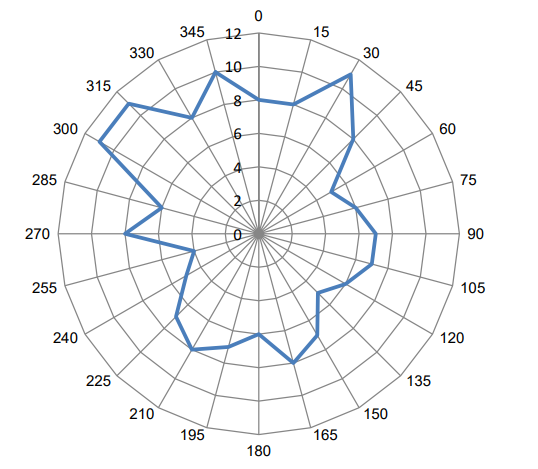
\includegraphics[width=0.65\textwidth]{Chap03/Figures/Antenna_Radiation_Pattren.PNG}
	\caption{Antenna Radiation Pattren}
	\label{fig:ANTENNA_RADIATION_PATTERN}
\end{figure}

% \subsection{PCB Meandered Inverted-F Antenna (PIFA)}

PIFA antennas are much more popular in Bluetooth Low Energy stack because of the small size low profile and cost-effective compared to the conventional dipole and ceramic chip antennas.
The proposed structure of the PIFA antenna is routed to gain all these advantages.
Replacing the conventional PCB line in PIFA with the meandering line and meandering shorting strip
improves the efficiency of the PIFA as well as the bandwidth. As a case study, the design and measurement results of the
proposed PIFA are presented \cite{PIFA2017Cheuk} in Figure\ref{fig:PIFA_Antenna_1}.


\begin{figure}[ht]
	\centering
	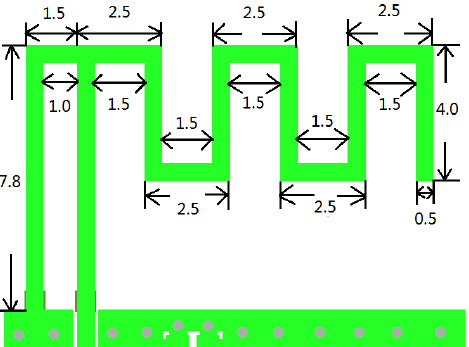
\includegraphics[width=0.65\textwidth]{Chap03/Figures/MIFA_Antenna.PNG}
	\caption{PCB Inverted Meandered F type Antenna }
	\label{fig:PIFA_Antenna_1}
\end{figure}




\subsection{PCB Meandered Inverted-F Antenna (PIFA)}

PIFA antennas are much more popular in Bluetooth Low Energy stack because of the small size low profile and cost-effective compared to the conventional dipole and ceramic chip antennas.
The proposed structure of the PIFA antenna is routed to gain all these advantages.
Replacing the conventional PCB line in PIFA with the meandering line and meandering shorting strip
improves the efficiency of the PIFA as well as the bandwidth. As a case study, the design and measurement results of the
proposed PIFA are presented \cite{PIFA2017Cheuk} in Figure\ref{fig:PIFA_Antenna_1}.


\begin{figure}[ht]
	\centering
	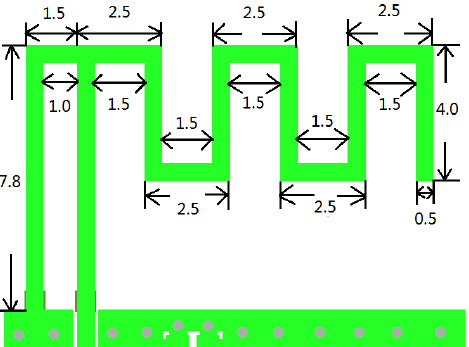
\includegraphics[width=0.65\textwidth]{Chap03/Figures/MIFA_Antenna.PNG}
	\caption{PCB Inverted Meandered F type Antenna }
	\label{fig:PIFA_Antenna_1}
\end{figure}